Database gestisce l'utilizzo del database tramite le classi DatabaseManager e derivate. La suddivisione rispecchia la rappresentazione dei dati all'interno della base di dati. In particolare:
\begin{itemize}
	\item \texttt{DatabaseExerciseManager}: permette le operazioni CRUD$^{*}$ e di ricerca degli esercizi;
	\item \texttt{DatabaseClassManager}: permette le operazioni CRUD e di ricerca delle classi;
	\item \texttt{DatabaseUserManager}: permette le operazioni CRUD e di ricerca degli User.
\end{itemize}

\begin{figure}[h]
	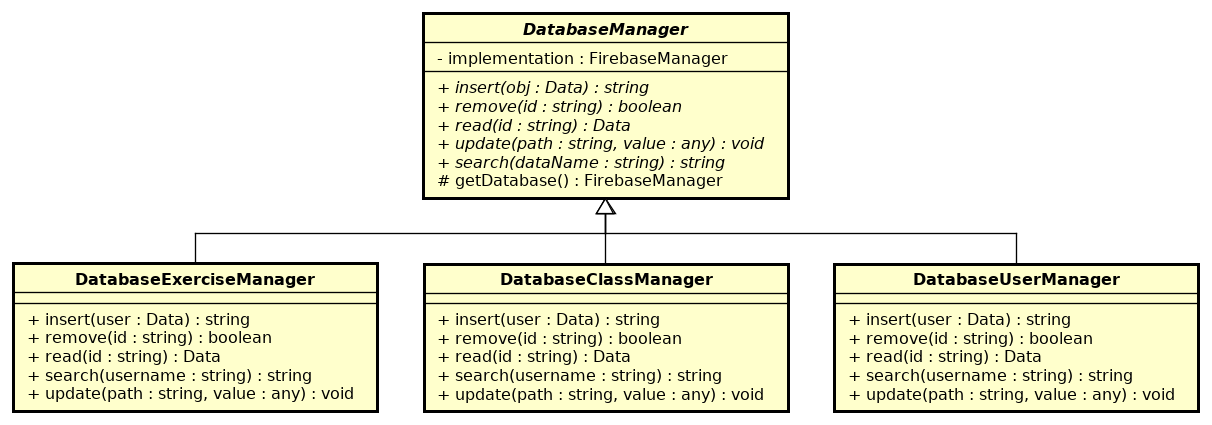
\includegraphics[scale=0.5]{images/DatabaseManager.png}
	\caption{Diagramma delle classi del package Database}
\end{figure}